% Options for packages loaded elsewhere
% Options for packages loaded elsewhere
\PassOptionsToPackage{unicode}{hyperref}
\PassOptionsToPackage{hyphens}{url}
\PassOptionsToPackage{dvipsnames,svgnames,x11names}{xcolor}
%
\documentclass[
  sn-basic,
]{sn-jnl}


\usepackage{xcolor}
\usepackage{amsmath,amssymb}
\setcounter{secnumdepth}{5}
\usepackage{iftex}
\ifPDFTeX
  \usepackage[T1]{fontenc}
  \usepackage[utf8]{inputenc}
  \usepackage{textcomp} % provide euro and other symbols
\else % if luatex or xetex
  \usepackage{unicode-math} % this also loads fontspec
  \defaultfontfeatures{Scale=MatchLowercase}
  \defaultfontfeatures[\rmfamily]{Ligatures=TeX,Scale=1}
\fi
\usepackage{lmodern}
\ifPDFTeX\else
  % xetex/luatex font selection
\fi
% Use upquote if available, for straight quotes in verbatim environments
\IfFileExists{upquote.sty}{\usepackage{upquote}}{}
\IfFileExists{microtype.sty}{% use microtype if available
  \usepackage[]{microtype}
  \UseMicrotypeSet[protrusion]{basicmath} % disable protrusion for tt fonts
}{}
\makeatletter
\@ifundefined{KOMAClassName}{% if non-KOMA class
  \IfFileExists{parskip.sty}{%
    \usepackage{parskip}
  }{% else
    \setlength{\parindent}{0pt}
    \setlength{\parskip}{6pt plus 2pt minus 1pt}}
}{% if KOMA class
  \KOMAoptions{parskip=half}}
\makeatother
% Make \paragraph and \subparagraph free-standing
\makeatletter
\ifx\paragraph\undefined\else
  \let\oldparagraph\paragraph
  \renewcommand{\paragraph}{
    \@ifstar
      \xxxParagraphStar
      \xxxParagraphNoStar
  }
  \newcommand{\xxxParagraphStar}[1]{\oldparagraph*{#1}\mbox{}}
  \newcommand{\xxxParagraphNoStar}[1]{\oldparagraph{#1}\mbox{}}
\fi
\ifx\subparagraph\undefined\else
  \let\oldsubparagraph\subparagraph
  \renewcommand{\subparagraph}{
    \@ifstar
      \xxxSubParagraphStar
      \xxxSubParagraphNoStar
  }
  \newcommand{\xxxSubParagraphStar}[1]{\oldsubparagraph*{#1}\mbox{}}
  \newcommand{\xxxSubParagraphNoStar}[1]{\oldsubparagraph{#1}\mbox{}}
\fi
\makeatother


\usepackage{longtable,booktabs,array}
\usepackage{calc} % for calculating minipage widths
% Correct order of tables after \paragraph or \subparagraph
\usepackage{etoolbox}
\makeatletter
\patchcmd\longtable{\par}{\if@noskipsec\mbox{}\fi\par}{}{}
\makeatother
% Allow footnotes in longtable head/foot
\IfFileExists{footnotehyper.sty}{\usepackage{footnotehyper}}{\usepackage{footnote}}
\makesavenoteenv{longtable}
\usepackage{graphicx}
\makeatletter
\newsavebox\pandoc@box
\newcommand*\pandocbounded[1]{% scales image to fit in text height/width
  \sbox\pandoc@box{#1}%
  \Gscale@div\@tempa{\textheight}{\dimexpr\ht\pandoc@box+\dp\pandoc@box\relax}%
  \Gscale@div\@tempb{\linewidth}{\wd\pandoc@box}%
  \ifdim\@tempb\p@<\@tempa\p@\let\@tempa\@tempb\fi% select the smaller of both
  \ifdim\@tempa\p@<\p@\scalebox{\@tempa}{\usebox\pandoc@box}%
  \else\usebox{\pandoc@box}%
  \fi%
}
% Set default figure placement to htbp
\def\fps@figure{htbp}
\makeatother





\setlength{\emergencystretch}{3em} % prevent overfull lines

\providecommand{\tightlist}{%
  \setlength{\itemsep}{0pt}\setlength{\parskip}{0pt}}





%%%% Standard Packages

\usepackage{graphicx}%
\usepackage{multirow}%
\usepackage{amsmath,amssymb,amsfonts}%
\usepackage{amsthm}%
\usepackage{mathrsfs}%
\usepackage[title]{appendix}%
\usepackage{xcolor}%
\usepackage{textcomp}%
\usepackage{manyfoot}%
\usepackage{booktabs}%
\usepackage{algorithm}%
\usepackage{algorithmicx}%
\usepackage{algpseudocode}%
\usepackage{listings}%

%%%%

\raggedbottom
\makeatletter
\@ifpackageloaded{caption}{}{\usepackage{caption}}
\AtBeginDocument{%
\ifdefined\contentsname
  \renewcommand*\contentsname{Table of contents}
\else
  \newcommand\contentsname{Table of contents}
\fi
\ifdefined\listfigurename
  \renewcommand*\listfigurename{List of Figures}
\else
  \newcommand\listfigurename{List of Figures}
\fi
\ifdefined\listtablename
  \renewcommand*\listtablename{List of Tables}
\else
  \newcommand\listtablename{List of Tables}
\fi
\ifdefined\figurename
  \renewcommand*\figurename{Figure}
\else
  \newcommand\figurename{Figure}
\fi
\ifdefined\tablename
  \renewcommand*\tablename{Table}
\else
  \newcommand\tablename{Table}
\fi
}
\@ifpackageloaded{float}{}{\usepackage{float}}
\floatstyle{ruled}
\@ifundefined{c@chapter}{\newfloat{codelisting}{h}{lop}}{\newfloat{codelisting}{h}{lop}[chapter]}
\floatname{codelisting}{Listing}
\newcommand*\listoflistings{\listof{codelisting}{List of Listings}}
\usepackage{amsthm}
\theoremstyle{plain}
\newtheorem{proposition}{Proposition}[section]
\theoremstyle{remark}
\AtBeginDocument{\renewcommand*{\proofname}{Proof}}
\newtheorem*{remark}{Remark}
\newtheorem*{solution}{Solution}
\newtheorem{refremark}{Remark}[section]
\newtheorem{refsolution}{Solution}[section]
\makeatother
\makeatletter
\makeatother
\makeatletter
\@ifpackageloaded{caption}{}{\usepackage{caption}}
\@ifpackageloaded{subcaption}{}{\usepackage{subcaption}}
\makeatother
\usepackage{bookmark}
\IfFileExists{xurl.sty}{\usepackage{xurl}}{} % add URL line breaks if available
\urlstyle{same}
\hypersetup{
  pdftitle={Tail Flexibility in the Degrees of Preferential Attachment Networks},
  pdfauthor={Thomas William Boughen; Clement Lee; Vianey Palacios Ramirez},
  pdfkeywords={networks, discrete extremes, degree distribution},
  colorlinks=true,
  linkcolor={blue},
  filecolor={Maroon},
  citecolor={Blue},
  urlcolor={Blue},
  pdfcreator={LaTeX via pandoc}}


\title[Tail Flexibility in the Degrees of Preferential Attachment
Networks]{Tail Flexibility in the Degrees of Preferential Attachment
Networks}

% author setup
\author[1]{\fnm{Thomas William} \sur{Boughen}}\author[1]{\fnm{Clement} \sur{Lee}}\author[1]{\fnm{Vianey Palacios} \sur{Ramirez}}
% affil setup
\affil[1]{\orgdiv{School of Mathematics, Statistics and
Physics}, \orgname{Newcastle University, UK}}

% abstract 

\abstract{Devising the underlying generating mechanism of a real-life
network is difficult as, more often than not, only its snapshots are
available, but not its full evolution. One candidate for the generating
mechanism is preferential attachment which, in its simplest form,
results in a degree distribution that follows the power law.
Consequently, the growth of real-life networks that roughly display such
power-law behaviour is commonly modelled by preferential attachment.
However, the validity of the power law has been challenged by the
presence of alternatives with comparable performance, as well as the
recent findings that the right tail of the degree distribution is often
lighter than implied by the body, whilst still being heavy. In this
paper, we study a modified version of the model with a flexible
preference function that allows super/sub-linear behaviour whilst also
guaranteeing that the limiting degree distribution has a heavy tail. We
relate the distributions tail heaviness directly to the model
parameters, allowing direct inference of the parameters from the degree
distribution alone.}

% keywords
\keywords{networks,  discrete extremes,  degree distribution}

\begin{document}
\maketitle


\section*{CL: Overall comments}\label{cl-overall-comments}
\addcontentsline{toc}{section}{CL: Overall comments}

\begin{enumerate}
\def\labelenumi{\arabic{enumi}.}
\tightlist
\item
  The introduction section is not quite clear and needs a lot of
  improvement, so here are my suggestions on the outline, in a hopefully
  more logical flow:

  \begin{enumerate}
  \def\labelenumii{\alph{enumii}.}
  \tightlist
  \item
    Start with the broad picture e.g.~that networks exist in many fields
    (name some for which you can cite applications), and that
    statistical methods are have been used to study networks. Some are
    for revealing the latent / underlying structures of the networks
    (stochastic block models), some are for explaining some response
    variables by network properties (ERGMs), and some are for
    postulating how the network grows and evolves (mechanistic models).
    Find some references, either the groundbreaking ones or
    comprehensive reviews to back this up.
  \item
    Introduce the general PA model as one of the mechanistic models.
    This will be a natural point to mention the rules (in terms as
    simple as possible) and introduce the preference function. Mention
    the special case when \(b(k)=k\) and cite \citet{Barabasi99}.
  \item
    Then talk about PA model and mechanistic models in general being
    useful to \textbf{simulate} networks but not be fitted to real data
    because usually only snapshots are available. This leads well into
    the point on the degree distribution being informative.
  \item
    Then in the paragraph starting ``When looking at \ldots{}'', point
    out that it is the BA model \citep{Barabasi99} that leads to a power
    law degree distribution.
  \item
    Then point out that while it's attempting to attribute to the BA
    model when degrees seemingly follow the power law, there are two
    main concerns: first, a general preference function doesn't lead to
    the power law \citep{krapivsky01}; second, some claim that a lot of
    real data don't actually follow the power law. Mention not only
    \citet{Broido_2019} but also responses to them e.g. \citet{vvvk19}.
  \item
    \citet{vvvk19} leads naturally to the point that extreme value
    methods have not been used in analysing degree distributions until
    recently, such as \citet{vvvk19} and \citet{lef24}. Not using these
    methods essentially downweights the deviation of the vertices with
    large degrees, which have far more influence on the network than
    those with small degrees, from the power law behaviour.
  \item
    Also mention Resnick's works (and others) on the crossroads of
    networks and extremes. Summarise what these papers do.
  \item
    Come back to the focus on the degree distribution, and point out
    that most methods, whether extremes are incorporated or not, are
    descriptive in the sense that no information about the preference
    function \(b(\cdot)\) is revealed, even if PA model was indeed the
    underlying mechanism.
  \item
    Then mention that this paper addresses that gap. Specifically,
    \textbf{given the degree distribution of the network assumed to come
    from the PA model, can we directly infer the model parameters?}
    While \citet{rudas07} have derived the limiting degree distribution
    in terms of \(b(\cdot)\) and its parameters, we build upon it by
    finding the class of preference functions that result in realistic
    tails (heavy but not as heavy as implied by the power law).
  \item
    Then go straight to the division of the rest of the paper, and
    conclude the introduction section. The remaining materials should
    mostly go to the next section, but you can retain some materials if
    you think they complement (or already address) the above points.
  \end{enumerate}
\item
  Rough outline of Section 2, which should be on the PA model and
  deriving the tail heaviness of the limiting degree distribution in
  terms of \(b(\cdot)\):

  \begin{enumerate}
  \def\labelenumii{\alph{enumii}.}
  \tightlist
  \item
    Start with the general description of the PA model. You can move
    here the paragraphs in the introduction section, starting with ``The
    network generative model \ldots{}'', ``Starting at time \ldots{}'',
    and ``Special cases of this model \ldots{}''. Most of what you have
    written up till the pmf can be kept.
  \item
    Next, first state that of interest is the tail heaviness (which here
    refers to the shape parameter of the (integer) GPD approximation of
    the tail). Then move here the paragraphs on \citet{shimura12} from
    the introduction.
  \item
    Then state proposition 2.1 and point to the Appendix for the proof.
  \item
    Next, we need a bit more discussion and explanation before stating
    that \(b(\cdot)\) has to be asymptotically linear for a heavy tail.
    First point out that this result covers and aligns with the
    previously obtained result i.e. \citet{krapivsky01}. This is pretty
    much the paragraph currently under Section 2.1, but with a better
    flow. You might even include the special case of the special case
    i.e.~\(b(k)=k+\epsilon\), to briefly illustrate how a tail heaviness
    of \(0.5\) is obtained for the BA model.
  \item
    Now, argue that \(b(\cdot)\) has to be (asymptotically) linear above
    a threshold, in order to have a positive tail heaviness, then
    introduce the proposed preference function as our model, with tail
    heaviness \(\beta/\lambda^{*}\).
  \item
    Conclude the section by saying that we will examine its property in
    the next Section (see next point).
  \end{enumerate}
\item
  The section could be called ``Preferential attachment with flexible
  heavy tail'', essentially making the subsection a section itself.

  \begin{enumerate}
  \def\labelenumii{\alph{enumii}.}
  \tightlist
  \item
    Most of the materials can be kept, and the form of the IGPD should
    be inserted when approximating the survival using Stirling's (not
    Sterling's) approximation. The survival of the IGPD was in the
    introduction but I suggest moving it here.
  \item
    The piecewise linear model doesn't add much, so I would consider
    excluding it unless there's a point e.g.~computational simplicity?
  \item
    I would conclude the section by moving the likelihood expression
    here, and say that the parameters can be inferred in a standard way,
    via the frequentist or Bayesian approach, as the likelihood is an
    explicit function of the parameters.
  \end{enumerate}
\item
  For simplicity, it's easier to use \(m=1\) throughout and only mention
  the general case \(m>1\) as future work in the discussion section.
  Also, it might be worth just calling the general preferential
  attachment model without the word ``general'' throughout, as it is
  unambiguous that it is the model with a flexible / general
  \(b(\cdot)\), while the BA model is the one with \(\b(k)=k+\epsilon\).
\item
  There are inconsistencies and duplications in various places, probably
  because you edited at one place and didn't update associated instances
  elsewhere. Do go back and forth when making edits.
\item
  The presentation can use many incremental improvements:

  \begin{enumerate}
  \def\labelenumii{\alph{enumii}.}
  \tightlist
  \item
    use \(k\) or \(n\) for the integer but not both, unless necessary
    and in a consistent way. There were places where \(n\) was used as
    the subject initially but it changed to \(k\).
  \item
    ensure that the text in plots are legible.
  \item
    when citing, use the parentheses correctly, as they have been used
    inappropriately; in Quarto syntax, the square brackets will
    automatically put the parentheses (similar to citep in LaTeX).
  \item
    ensure that the maths don't over the linewidth.
  \item
    introduce the full term with the acronym in parentheses when using
    it for the first time, e.g.~GPA.
  \item
    some references of equations are not working e.g.~eq-surv?
  \item
    unless necessary, avoid strong adverbs / adjectives.
  \end{enumerate}
\item
  It seems that you version control all the files, which I won't
  recommend. Only track the files that you manually change, not the
  generated ones (cache, pdf, and tex unless you manually created one).
  This will facilitate the reproducibility. I have removed the generated
  files in my branch.
\item
  Consider creating subfolders to store the results, data, figures, etc.
  This will streamline your file structure. I have accordingly edited
  the R scripts so that if you run them, the rds files will be stored in
  results/.
\item
  Accents in names in bib / tex / qmd might not work on some computers.
  Here's the conversion chart: https://www.bibtex.org/SpecialSymbols/
\end{enumerate}

\section{Introduction}\label{sec-intro}

The degree distribution of a network can be very informative about the
networks structure, giving some understanding about the inequality in
the influence of the nodes. Often the degree distribution is one of the
simplest places to look when trying to understand this, as the full
evolution of the network is usually not available. This makes modelling
the degree distribution an important topic in research with
contributions such as {[}ref{]}.

When looking at the degree distributions of real networks, a power law
is an attractive option to use when modelling as it is seemingly
observed in a lot of networks. Fitting the discrete power law to the
degree distribution come with the added benefit of suggesting
preferential attachment as the generating mechanism since it has been
shown to generate networks with a power law degree distribution.

Whether the power law is adequate for real degree distributions has
become a heated debate, with alternatives such as \citet{Broido_2019}
seeming to outperform the power law in some cases. Additionally,
\citet{lef24} find that for many real degree distributions the body may
follow a power law, the right tail does not or at least seems to be
lighter than is implied by the body whilst still being heavy. One method
for modelling the tail of the degree distributions of real networks is
to use a discretised variation of the generalised Pareto distribution
(GPD) usually dubbed the Integer GPD (GPD) where
\(X|X>v \sim \mathrm{IGPD}(\xi,\sigma,v)\) is defined by the survival:

\[
\Pr(X> x|X> v) = \left(\frac{\xi(x-v)}{\sigma} + 1\right)^{-1/\xi},\qquad x=v+1,v+2,\ldots
\] for \(v\in\mathbb Z^+, \sigma>0,\xi\in \mathbb R\).

{[}CL: Is the precise form of the IGPD needed here? The big picture is
probably more important (point 3f in overall comments){]}

\citet{shimura12} introduces a quantity that will help in determining
what domain of attraction a discrete distribution belongs to, that is:

For a distribution \(F\) with survival function \(\bar F\) and some
\(n\in\mathbb Z^+\) let:

\[
\Omega(F,n) = \left(\log\displaystyle\frac{\bar F (n+1)}{\bar F (n+2)}\right)^{-1} - \left(\log\displaystyle\frac{\bar F (n)}{\bar F (n+1)}\right)^{-1}
\]

\citet{shimura12} then states that if
\(\lim_{n\rightarrow\infty} \Omega(F,n) = 1/\alpha\) (\(\alpha>0\)),
then \(F\) is heavy tailed with \(\bar F(n) \sim n^{-\alpha}\).
Additionally, if \(\lim_{n\rightarrow\infty} \Omega(F,n) = 0\) then the
distribution is light tailed.

\citep[CL: The results of][ could be moved closer to Proposition 2.1. In
the introduction, if you want to include \citet{shimura12}, you can
mention the paper in passing, when outlining your approach, e.g.~``Using
the results by \citet{shimura12}, we derive the tail index / heaviness
of the limiting degree distribution of the GPA model \citep{rudas07}.
This informs us the precise class of preference functions that result in
flexible heavy tail.'']{shimura12}

These models that seem to outperform the power law do not however come
with the added benefit of suggesting a generating mechanism for the
networks in the same way the power law does. Efforts to make the
preferential attachment model more flexible have not yet remedied this
issue with \citet{krapivsky01} finding that using a sub/super-linear
preference function yields a Weibull tail and a degenerate network,
where one vertex eventually gains all new edges, respectively.

The network generative model that we will be focussing on in this paper
is dubbed General Preferential Attachment in \citet{rudas07} and is
defined as follows:

Starting at time \(t=0\) with an initial network of \(m\) vertices that
each have no edges, at times \(t=1,2,\ldots\) a new vertex is added to
the network bringing with it \(m\) directed edges (with the new vertex
as the source); the target for each of these edges are selected from the
vertices already in the network with weights proportional to some
function \(b\) of their degree.

Special cases of this model include the Barabási-Albert (BA) model when
\(b(k) = k+\varepsilon\), which leads to a power-law degree distribution
with index 2 and the Uniform Attachment (UA) model where \(b(k)=c\)
leading to a degree distribution in the Gumbel maximum domain of
attraction.

Estimating the preference function used by network generative models
like this is of great interest, with the potential to provide a deeper
understanding of the relationships between the vertices in the network.
Several papers and an R package (\texttt{PAfit}) have been dedicated to
estimating the preference function that may have been used when a
network was growing; one thing all these have in common is requiring
access to a networks evolution data, something that is not always
readily available or feasible to access. A method for estimating a
preference function without this data available would be extremely
useful.

\citet{rudas07} introduces theoretical results for this model with a
general preference function in the cases that the network being
generated is a tree (\(m=1\)); presenting an opportunity to design a
preference function that will capture the behaviours observed in the
degree distributions of real networks. Since they provide theoretical
results for the limiting degree distribution, a model of this form would
be able to be fitted to the degree distributions of real networks where
the full evolution is not available, only a snapshot.

The rest of this paper is as follows: Section~\ref{sec-gpa} looks at the
theoretical limiting behaviour of a GPA model when \(m=1\) according to
the results from \citet{rudas07}, going on to introduce a flexible class
of preference functions that can guarantee a heavy tailed degree
distribution while still being flexible in the body.
Section~\ref{sec-rec} shows that the preference function parameters can
be fairly well recovered from the degree distributions of networks
simulated from the GPA model using various functions of the class
introduced in Section~\ref{sec-gpa}. Having shown that for simulated
data the model parameters are recoverable from the degree distribution
alone, Section~\ref{sec-real} builds upon this and attempts to fit the
model to degree distributions of real networks; modelling not only the
degree distribution itself but also the estimates for the parameters of
the preference function assuming the networks evolved according to the
GPA scheme. Section~\ref{sec-conc} discusses the main results, proposes
future work and concludes the paper.

\section{General Preferential Attachment Model}\label{sec-gpa}

In this section, we introduce a general preferential attachment model,
with the focus on the limiting degree distribution as a function of the
preference function \(b(\cdot)\) where each vertex brings with it \(m\)
edges. This preference function is subject to the following conditions:

\[
b:\mathbb N \mapsto \mathbb R^+\setminus\{0\},
\]

\begin{equation}\phantomsection\label{eq-condb2}{
\sum_{k=0}^\infty\frac{1}{b(k)} = \infty.
}\end{equation}

Given these two conditions an expression for the survival of the
limiting degree distribution can be found in the case that \(m=1\);
obtained by considering a branching process that is equivalent to the
growth of the network, as in \citet{rudas07}. Theorem 1 from
\citet{rudas07} states that for the tree \(\Upsilon(t)\) at time \(t\):

\[
\lim_{t\rightarrow\infty}\frac{1}{|\Upsilon(t)|}\sum_{x\in\Upsilon(t)}\varphi(\Upsilon(t)_{\downarrow x}) = \lambda^* \int_0^\infty e^{-\lambda^* t}\mathbb E\left[\varphi(\Upsilon(t))\right]dt
\] where \(\lambda^*\) satisfies \(\hat\rho(\lambda^*)=1\). (CL:
\(\hat{\rho}\) has not been defined yet.)

The limiting survival can be viewed as the limit of the empirical
proportion of vertices with degree over a threshold \(k\), that is:

\[
\bar F(k) = \lim_{t\rightarrow\infty}\frac{\sum_{x\in\Upsilon(t)}\mathbb I\left\{\text{deg}(x,\Upsilon(t)_{\downarrow x})>k\right\}}{\sum_{x\in\Upsilon(t)} 1}
\] which by the previously stated theorem can also be written as:

\[
\bar F(k) = \frac{\int_0^\infty e^{-\lambda^* t}\mathbb E\left[\mathbb I\left\{\text{deg}(x,\Upsilon(t))>k\right\}\right]dt}{\int_0^\infty e^{-\lambda^* t}dt} = \prod_{i=0}^k\frac{b(i)}{\lambda^* + b(i)}.
\] Using the fact that \(f(k) = \bar F(k-1) - \bar F(k)\) the
probability mass function (pmf) is

\[
f(k) = \frac{\lambda^*}{\lambda^* + b(k)}\prod_{i=0}^{k-1}\frac{b(i)}{\lambda^*+b(i)},\qquad k\in\mathbb N,
\]

which aligns with the result from \citet{rudas07}, where the expression
is derived using the same branching process results.

Using results from \citet{shimura12}, the domain of attraction of this
limiting degree distribution can be found.

\begin{proposition}[]\protect\hypertarget{prp-omega}{}\label{prp-omega}

If \(b(k) \rightarrow \infty\) as \(k\rightarrow \infty\) then \[
\bar F(k) = \prod_{i=0}^k\frac{b(i)}{\lambda^* + b(i)}
\] and

\[
\lim_{k\rightarrow\infty}\Omega(F,k) = \lim_{k\rightarrow\infty}\frac{b(k+1)-b(k)}{\lambda^*}.
\]

\end{proposition}

Proposition~\ref{prp-omega} implies that the only way to obtain a heavy
tailed degree distribution using a non-decreasing preference function is
to have that preference function be asymptotically linear. The next
subsection focuses on a particular class of these preference functions
that provide flexible behaviour but guarantee a heavy tail.

\subsection{Preferential Attachment with flexible heavy
tail}\label{sec-model}

In \citet{krapivsky01}, a preference function of the form
\(k^\alpha +\varepsilon\) has been considered. However, it has been
noted that super-linear preferential attachment (\(\alpha > 1\)) leads
to a degenerate limiting degree distribution where at some point one
vertex gains the connection (CL: edge?) from every vertex that joins the
network, additionally sub-linear preferential attachment (\(\alpha <1\))
has been shown to lead to a light tailed limiting degree distribution.
Consider a preference function of the form:

\[
b(k) = \begin{cases}
k^\alpha + \varepsilon,&k<k_0,\\
k_0^\alpha + \varepsilon + \beta(k-k_0), &k\ge k_0,
\end{cases}
\] for \(\alpha,\beta, \varepsilon>0\) and \(k_0\in\mathbb N\).

Using a preference function with guaranteed linear behaviour in the
limit, allows for the inclusion of sub/super linear behaviour without
losing the heavy tails or ending up with a degenerate degree
distribution.

The limiting degree distribution resulting from using a preference
function of this form can be found to have survival:

\begin{equation}\phantomsection\label{eq-polysurv}{
\bar F(k) = \begin{cases}
\displaystyle\prod_{i=0}^{k}\frac{i^\alpha + \varepsilon}{\lambda^*+i^\alpha + \varepsilon},&k<k_0,\\
\displaystyle\left(\prod_{i=0}^{k_0-1}\frac{i^\alpha + \varepsilon}{\lambda^*+i^\alpha + \varepsilon}\right)\frac{\Gamma(\lambda^*+k_0^\alpha + \varepsilon)/\beta)}{\Gamma\left((k_0^\alpha + \varepsilon)/\beta\right)} \frac{\Gamma\left(k-k_0 + 1 +\frac{k_0^\alpha + \varepsilon}{\beta}\right)}{\Gamma\left(k-k_0 + 1 +\frac{\lambda^* +k_0^\alpha + \varepsilon}{\beta}\right)},&k\ge k_0,
\end{cases}
}\end{equation}

with \(\lambda^*\) satisfying \(\hat{\rho}(\lambda^{*})=1\), where

\[
\hat\rho(\lambda) = \sum_{n=0}^{k_0}\prod_{i=0}^{n-1}\frac{i^\alpha + \varepsilon}{\lambda+i^\alpha + \varepsilon} + \left(\frac{k_0^\alpha + \varepsilon}{\lambda-\beta}\right)\prod_{i=0}^{k_0-1}\frac{i^\alpha + \varepsilon}{\lambda + i^\alpha + \varepsilon} = 1,
\]

which has to be solved numerically for most parameter choices. Note that
\(\lambda\) has to be greater than \(\beta\) since when
\(\lambda\le \beta\) the infinite sum diverges. (CL: Where is the
infinite sum?)

Some examples of what the degree distribution looks like are shown below
in Figure~\ref{fig-polylinsurv}:

\begin{figure}[H]

\centering{

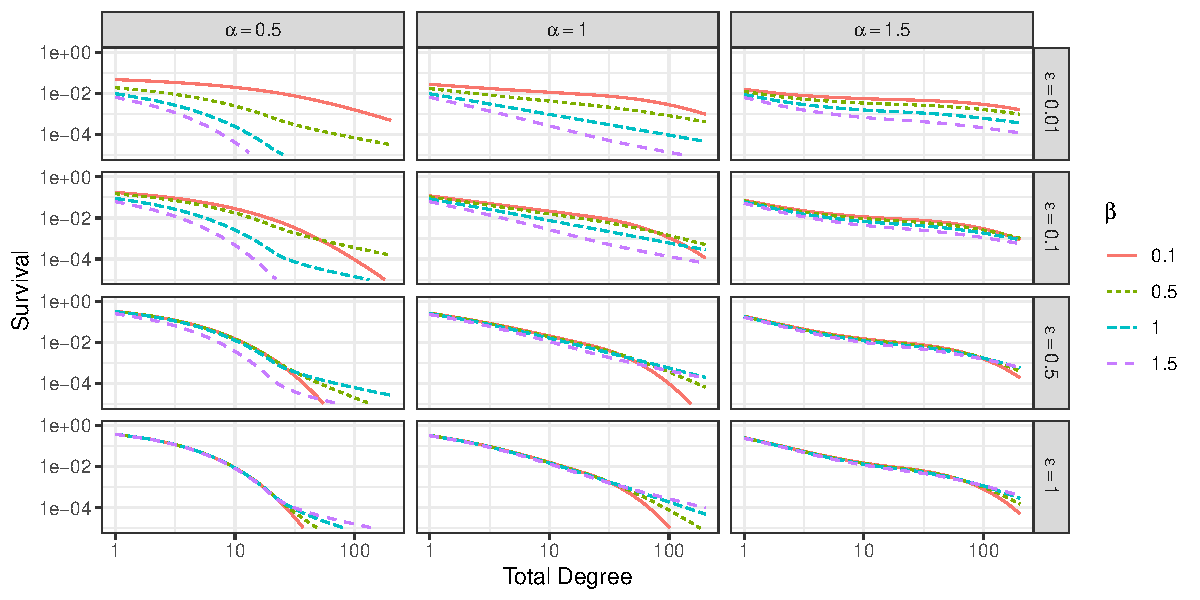
\includegraphics[width=0.95\linewidth,height=\textheight,keepaspectratio]{paper_files/figure-pdf/fig-polylinsurv-1.pdf}

}

\caption{\label{fig-polylinsurv}Theoretical survival distributions of
the limiting degree distributions, according to various combinations of
\((\alpha, \beta, \varepsilon)\) and \(k_0=20\) of the proposed
preferential attachment model.}

\end{figure}%

Applying Stirling's approximation of the gamma function to the second
case of Equation~\ref{eq-polysurv}, we obtain, for \(k\geq k_0\),

\[
\bar F(k) 
%\begin{cases}
%=\displaystyle\prod_{i=0}^{k}\frac{i^\alpha + \varepsilon}{\lambda^*+i^\alpha + \varepsilon},&k<k_0,\\
\displaystyle\approx \left(\prod_{i=0}^{k_0-1}\frac{i^\alpha + \varepsilon}{\lambda^*+i^\alpha + \varepsilon}\right) \left(\frac{\beta(k+1-k_0)}{k_0^{\alpha}+\varepsilon} + 1\right)^{-\lambda^*/\beta},%&k\ge k_0,
%\end{cases}
\] which is the survival function of the
\(\text{IGPD}\displaystyle\left(\frac{\beta}{\lambda^*}, \frac{k_0^\alpha + \varepsilon}{\lambda^*},k_0-1\right)\)
distribution. This means that, above the threshold of the piecewise
preference function, the limiting degree distribution can be
approximated by the IGPD with shape parameter \(\beta/\lambda^{*}\).

To assess the quality of the approximation, the conditional survivals
are shown in Figure~\ref{fig-approx_surv} in colour and their IGPD
approximations are shown in grey. The approximation seems to hold up
fairly well even for large degrees.

\begin{figure}[H]

\centering{

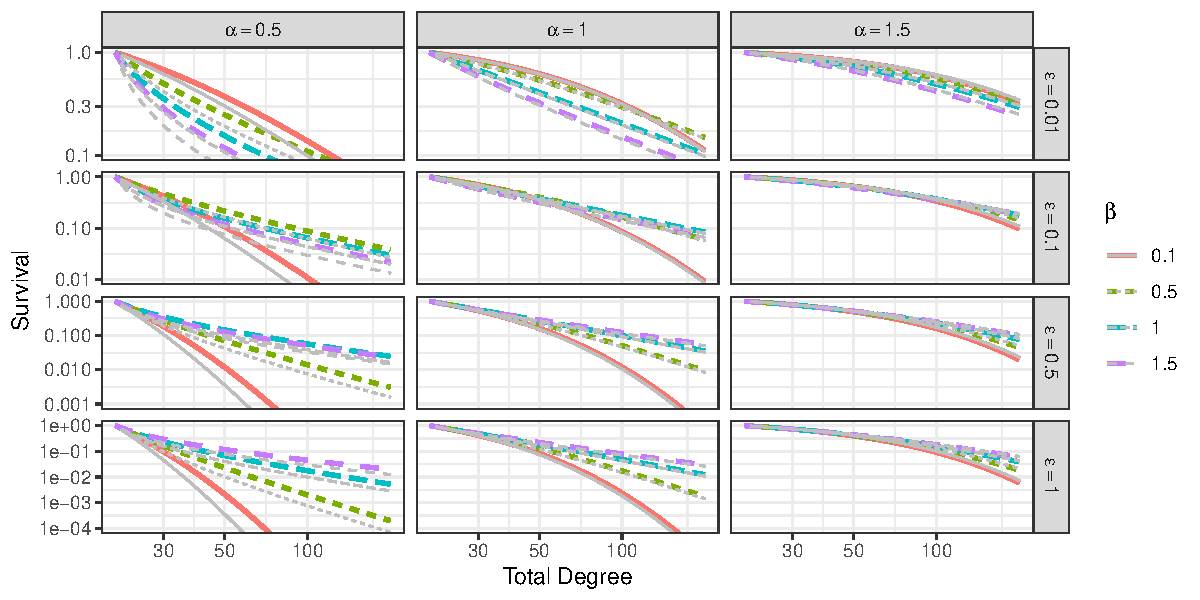
\includegraphics[width=0.95\linewidth,height=\textheight,keepaspectratio]{paper_files/figure-pdf/fig-approx_surv-1.pdf}

}

\caption{\label{fig-approx_surv}Theoretical conditional survivals (grey)
alongside their IGPD approximations (coloured).}

\end{figure}%

Since \(\beta>0\), the shape parameter of the IGPD is positive and thus
the distribution is heavy tailed. Additionally the value of the shape
parameter \(\xi\) is shown in Figure~\ref{fig-polyheat} for various
parameter choices:

\begin{figure}[H]

\centering{

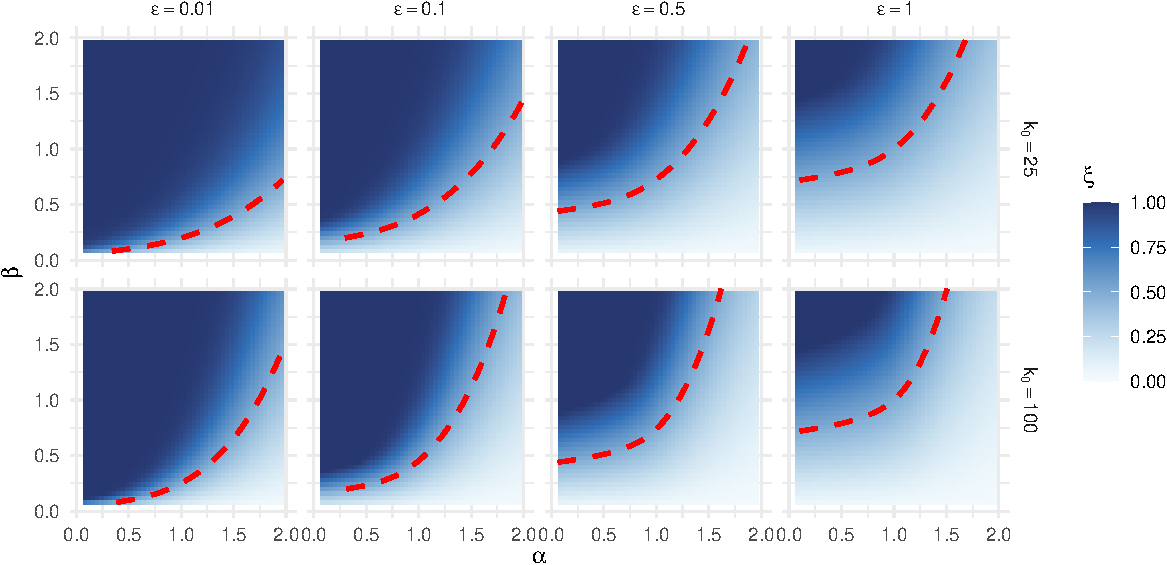
\includegraphics[width=0.95\linewidth,height=\textheight,keepaspectratio]{paper_files/figure-pdf/fig-polyheat-1.pdf}

}

\caption{\label{fig-polyheat}Heatmaps of \(\xi\) for various
combinations of the parameters of the proposed model.}

\end{figure}%

The darker regions on the heat maps correspond to a heavier tail and the
lighter to a lighter tail, the red dashed line shows combinations of
\(\alpha\) and \(\beta\) that produce a limiting degree distribution
with the same tail heaviness as the Barabási-Albert model, \(\xi=0.5\).

\subsubsection{Piecewise Linear Model}\label{piecewise-linear-model}

When \(\alpha = 1\) the preference function simplifies to a piecewise
linear function with \(\beta\) representing the ratio of the gradients
of the two components:

\[
b(k) = \min(k,k_0) + \varepsilon + \mathbb I\{k\ge k_0\}\beta(k-k_0)
\] for some \(\beta, \varepsilon, k_0>0\).

Following Equation~\ref{eq-polysurv} the limiting degree distribution
is:

\begin{equation}\phantomsection\label{eq-linsurv}{
\bar F(k) = \begin{cases}
\displaystyle\frac{\Gamma(\lambda^*+\varepsilon)\Gamma(k+1+\varepsilon)}{\Gamma(\varepsilon)\Gamma(k+1+\lambda^*+\epsilon)},&k<k_0,\\
\displaystyle\frac{\Gamma(\lambda^*+\varepsilon)\Gamma(k_0+\varepsilon)}{\Gamma(\varepsilon)\Gamma(k_0+\lambda^*+\varepsilon)}\times \frac{\Gamma\left(\frac{k_0+\varepsilon+\lambda^*}{\beta}\right)}{\Gamma\left(\frac{k_0+\varepsilon}{\beta}\right)}\times\frac{\Gamma\left(k-k_0 + \frac{k_0+\varepsilon}{\beta}+1\right)}{\Gamma\left(k-k_0 + \frac{k_0+\varepsilon+\lambda^*}{\beta}+1\right)},&k\ge k_0.
\end{cases}
}\end{equation}

Similar to the general case, the survival function can be approximated
by:

\[
\bar F(k) \approx \begin{cases}
\displaystyle\frac{\Gamma(\lambda^*+\varepsilon)}{\Gamma(\varepsilon)} (1+\varepsilon)^{\lambda^*}\left(\frac{k}{1+\varepsilon} + 1\right)^{-\lambda^*},&k<k_0,\\
\displaystyle\frac{\Gamma(\lambda^*+\varepsilon)\Gamma(k_0+\varepsilon)}{\Gamma(\varepsilon)\Gamma(k_0+\lambda^*+\varepsilon)}\times\left(\frac{\beta(k+1-k_0)}{k_0+\varepsilon} + 1\right)^{-\lambda^*/\beta},&k\ge k_0.
\end{cases}
\]

Some examples of the limiting degree distributions are shown in the
central column of Figure~\ref{fig-polylinsurv}.

\section{Simulation study}\label{sec-rec}

This section aims to show that the parameters of the model in
Section~\ref{sec-model} can be recovered from the degree distribution of
a network simulated from it.

The procedure for recovering the parameters begins with simulating a
network from the model with \(N=100,000\) vertices and \(m=1\) given
some set of parameters
\(\pmb\theta = (\alpha, \beta, \varepsilon, k_0)\), obtaining the degree
counts in the form of a vector of degrees \(\pmb x = (1,2,\ldots,M)\)
and the number of vertices with those degrees \(\pmb n\) where \(M\) is
the maximum degree. However, when it comes to fitting this model to real
data in the next section, small degrees are extremely influential and
will often cause the model to have a bad fit even though the rest of the
data looks similar to that of the simulations; truncating the data above
some value, say \(l<k_0\), should allow the model to be more effectively
fitted. This accounts in some way for the fact that this model only
applies to trees, and could not possibly capture the behaviour for nodes
with small degrees. Using the p.m.f derived in \citet{rudas07}, the
likelihood given that \(x_i \ge l\) for all \(i =1,2,\ldots,M\) is:

\begin{align*}
L(\pmb x,\pmb n | \pmb \theta) = \left(\frac{\lambda^*}{\lambda^*+\varepsilon}\right)^{n_0}\left(\prod_{j=l}^{k_0-1}\frac{j^\alpha +\varepsilon}{\lambda^* + j^\alpha +\varepsilon}\right)^{\left(\sum_{x_i\ge k_0}n_{x_i}\right)} \prod_{l \le x_i<k_0}\left(\frac{\lambda^*}{\lambda^* +x_i^\alpha + \varepsilon } \prod_{j=l}^{k_0-1}\frac{j^\alpha + \varepsilon}{\lambda^* + j^\alpha + \varepsilon}\right)^{n_i}\\ \times \prod_{x_i\ge k_0}\left(\frac{\text{B}(x_i-k_0 + (k_0^\alpha + \varepsilon)/\beta,1+\lambda^*/\beta)}{\text{B}((k_0^\alpha + \varepsilon)/\beta,\lambda^*/\beta)}\right)^{n_i}
\end{align*}

where \(B(y,z)\) is the the beta function.

This likelihood allows inference to be made about the parameters using a
Bayesian approach using the priors:

\begin{align*}
\alpha&\sim \text{Ga}(1,0.01),\\
\beta &\sim  \text{Ga}(1,0.01),\\
k_0 &\sim \text{U}(1,10,000),\\
\varepsilon &\sim \text{Ga(1,0.01)},
\end{align*}

to obtain a posterior distribution that can then be used in an adaptive
Metropolis-Hastings Markov chain Monte Carlo (MCMC) algorithm to obtain
posterior samples. The results of this inference are shown in
Figure~\ref{fig-rec1} and Figure~\ref{fig-rec2}. For these simulated
networks \(l=0\).

\begin{figure}[H]

\centering{

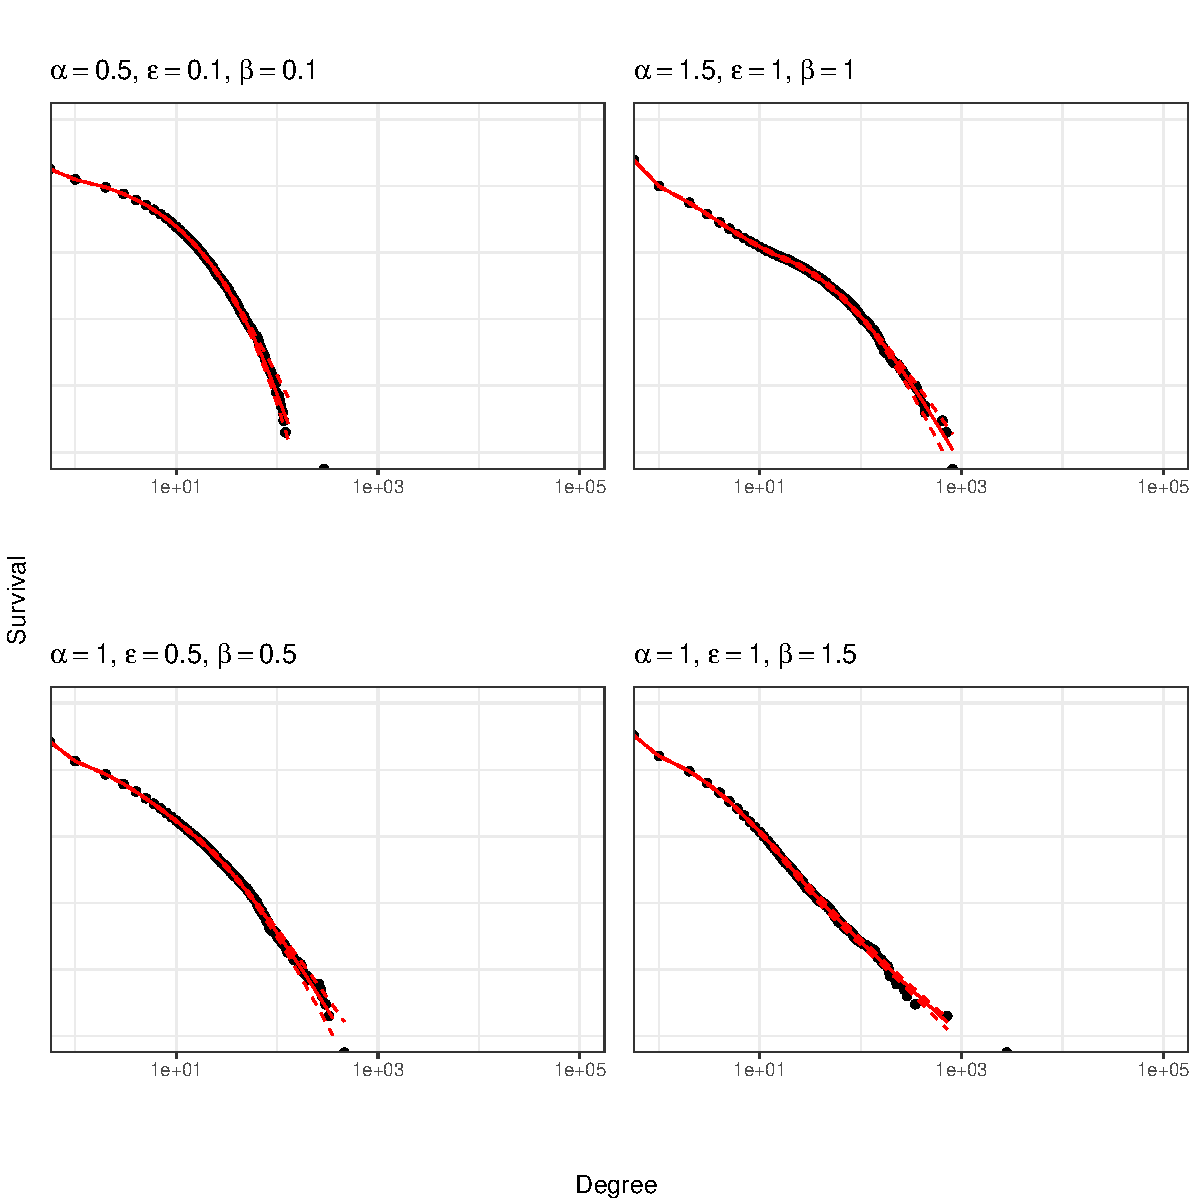
\includegraphics[width=0.95\linewidth,height=\textheight,keepaspectratio]{paper_files/figure-pdf/fig-rec1-1.pdf}

}

\caption{\label{fig-rec1}Posterior estimates of survival function for
data simulated from the proposed model with various combinations of
(\(\alpha,\beta,\varepsilon\)) and \(k_0=20\).}

\end{figure}%

\begin{figure}[H]

\centering{

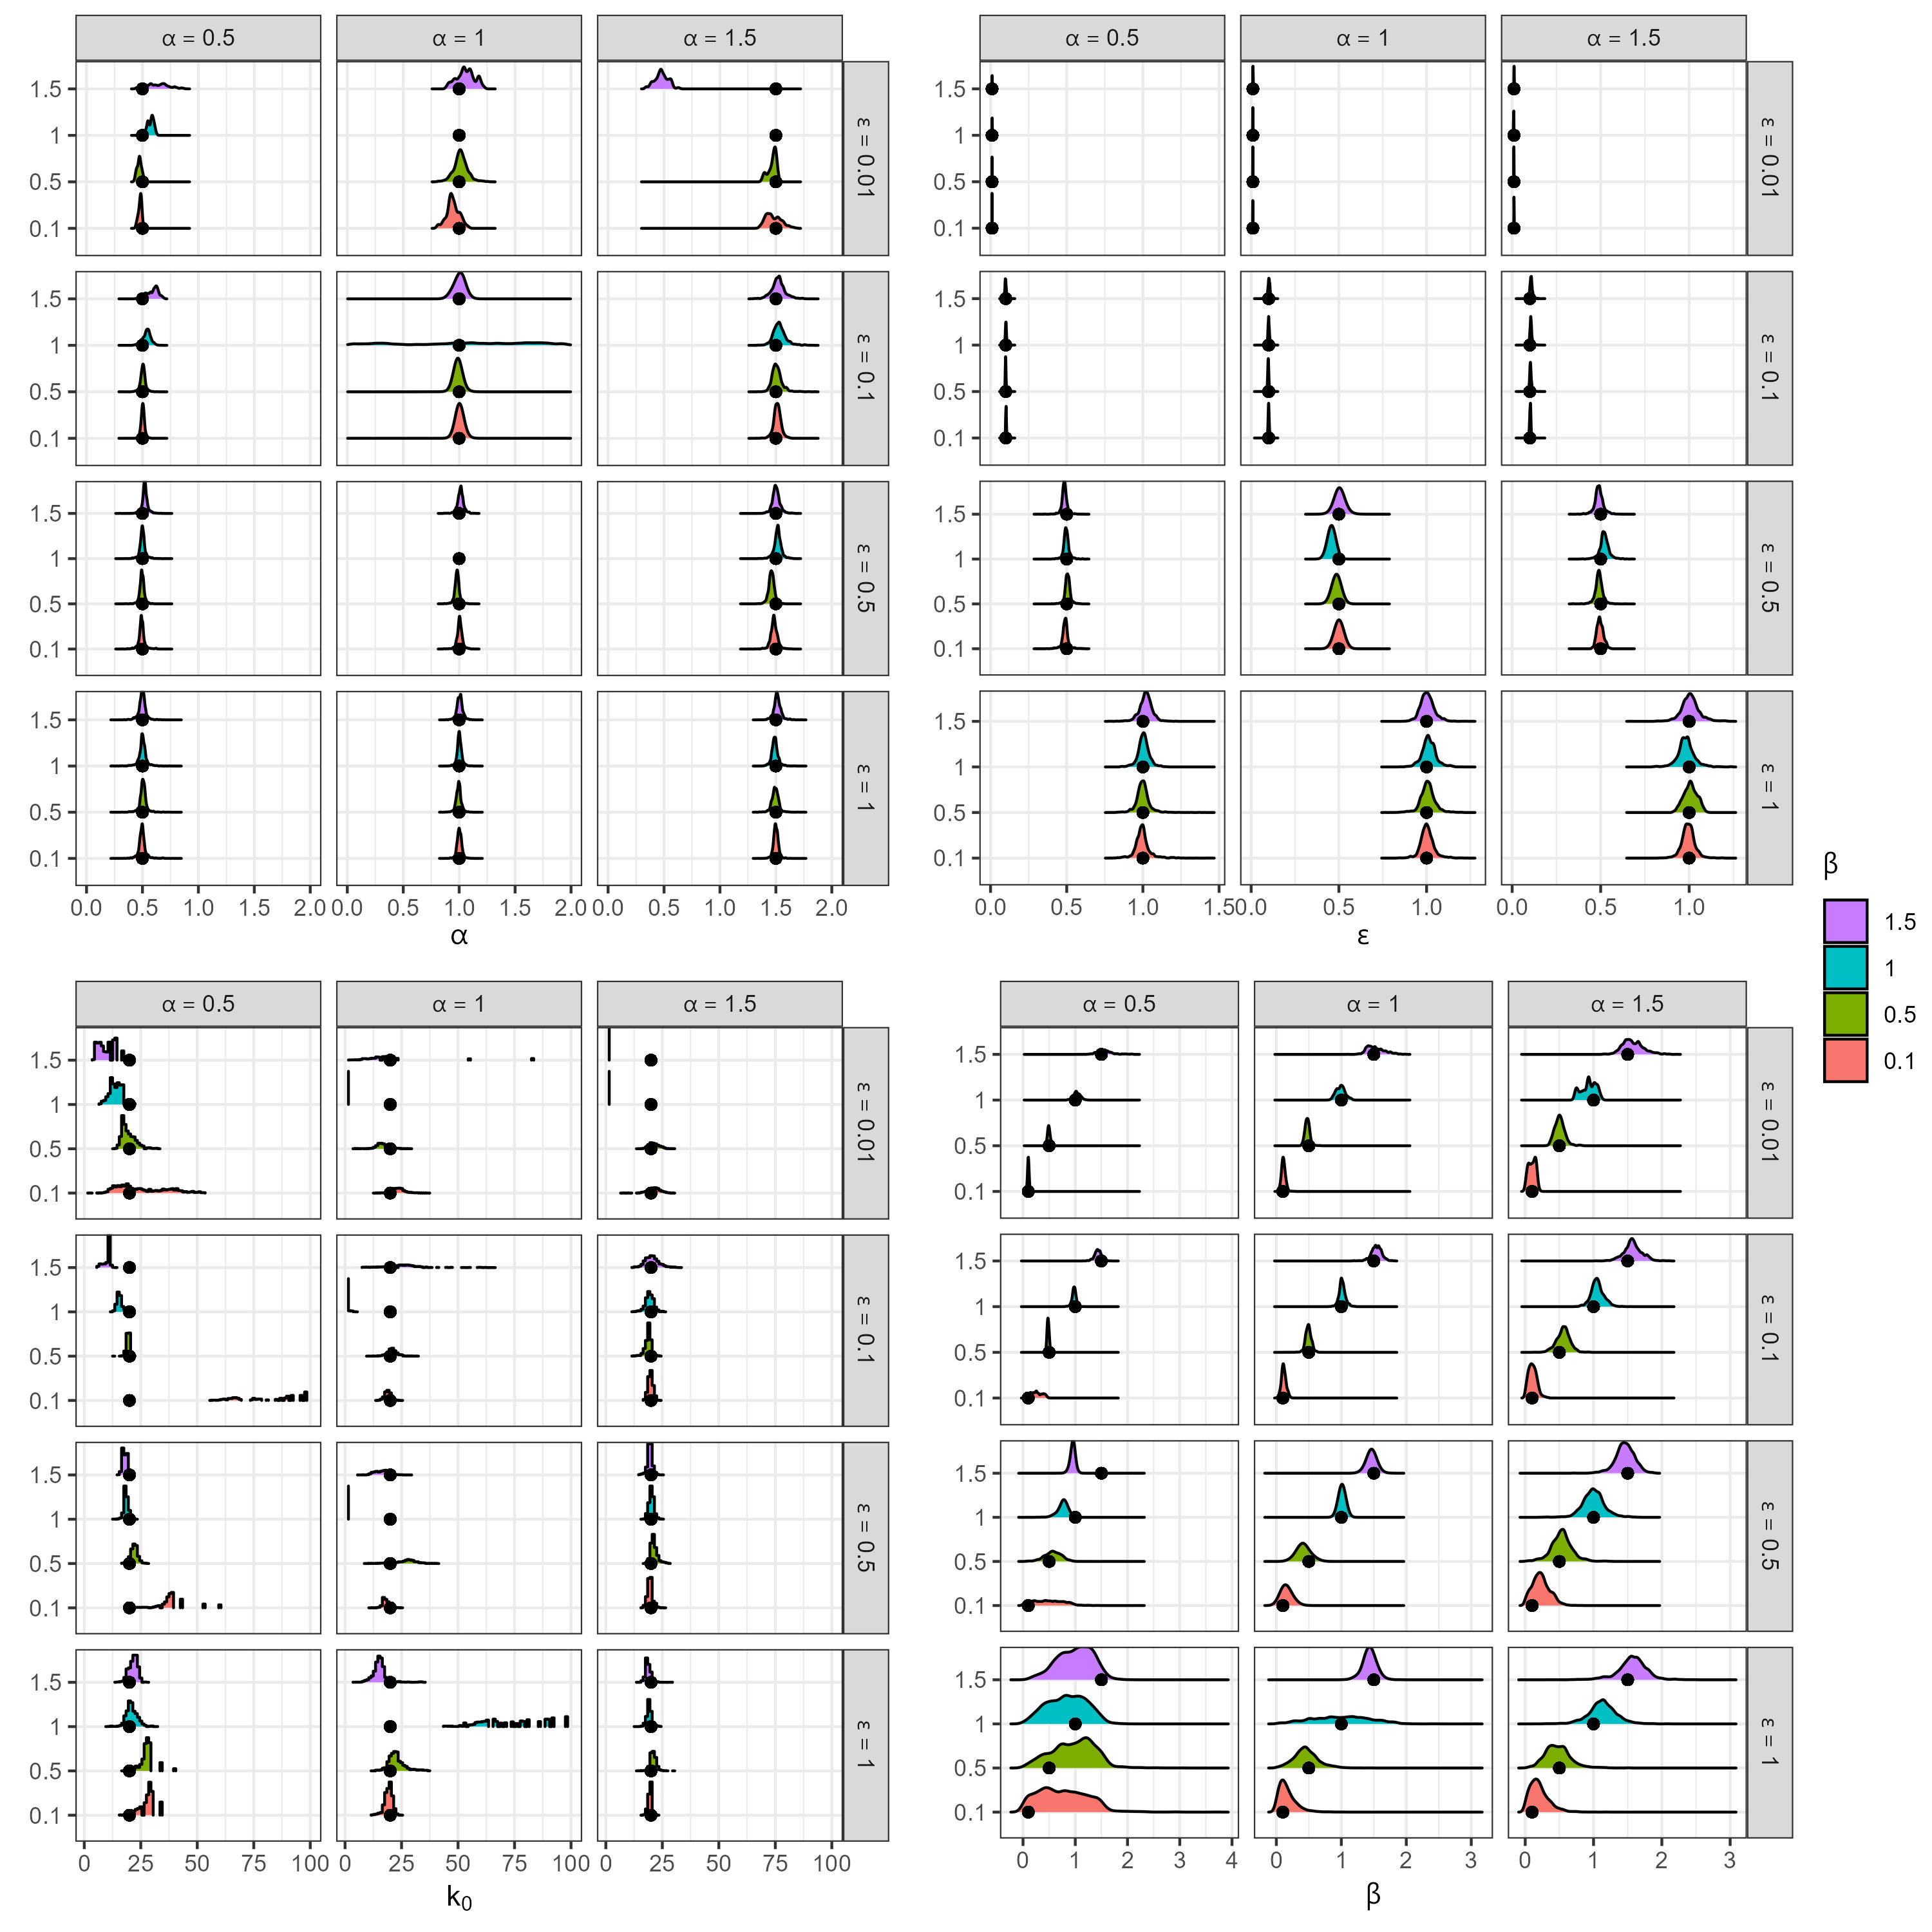
\includegraphics[width=0.8\linewidth,height=\textheight,keepaspectratio]{mcmc_plot.jpg}

}

\caption{\label{fig-rec2}Posterior estimates of parameters for data
simulated from the proposed model with various combinations of
(\(\alpha\),\(\beta\),\(\varepsilon\)) and \(k_0=20\).}

\end{figure}%

Figure~\ref{fig-rec1} and Figure~\ref{fig-rec2} demonstrate that using
this methodology it is possible to recover the model parameters fairly
well from only the final degree distribution of a simulated network.
This indicates that the method may also be able to be applied to the
degree distributions of real networks, estimating the model parameters
assuming they evolved according to the GPA scheme.

\section{Application to Real Data}\label{sec-real}

Turning now to real data, the goal is to fit the model to the degree
distributions of real networks from various sources. {[}describe
networks being used{]}. Alongside fitting this model to the degree
distributions, we then compare the fit to that of an mixture
distribution that was used in \citet{lef24} and is similar to others
that have been used to model degree distributions {[}others{]}.

\begin{figure}[H]

\centering{

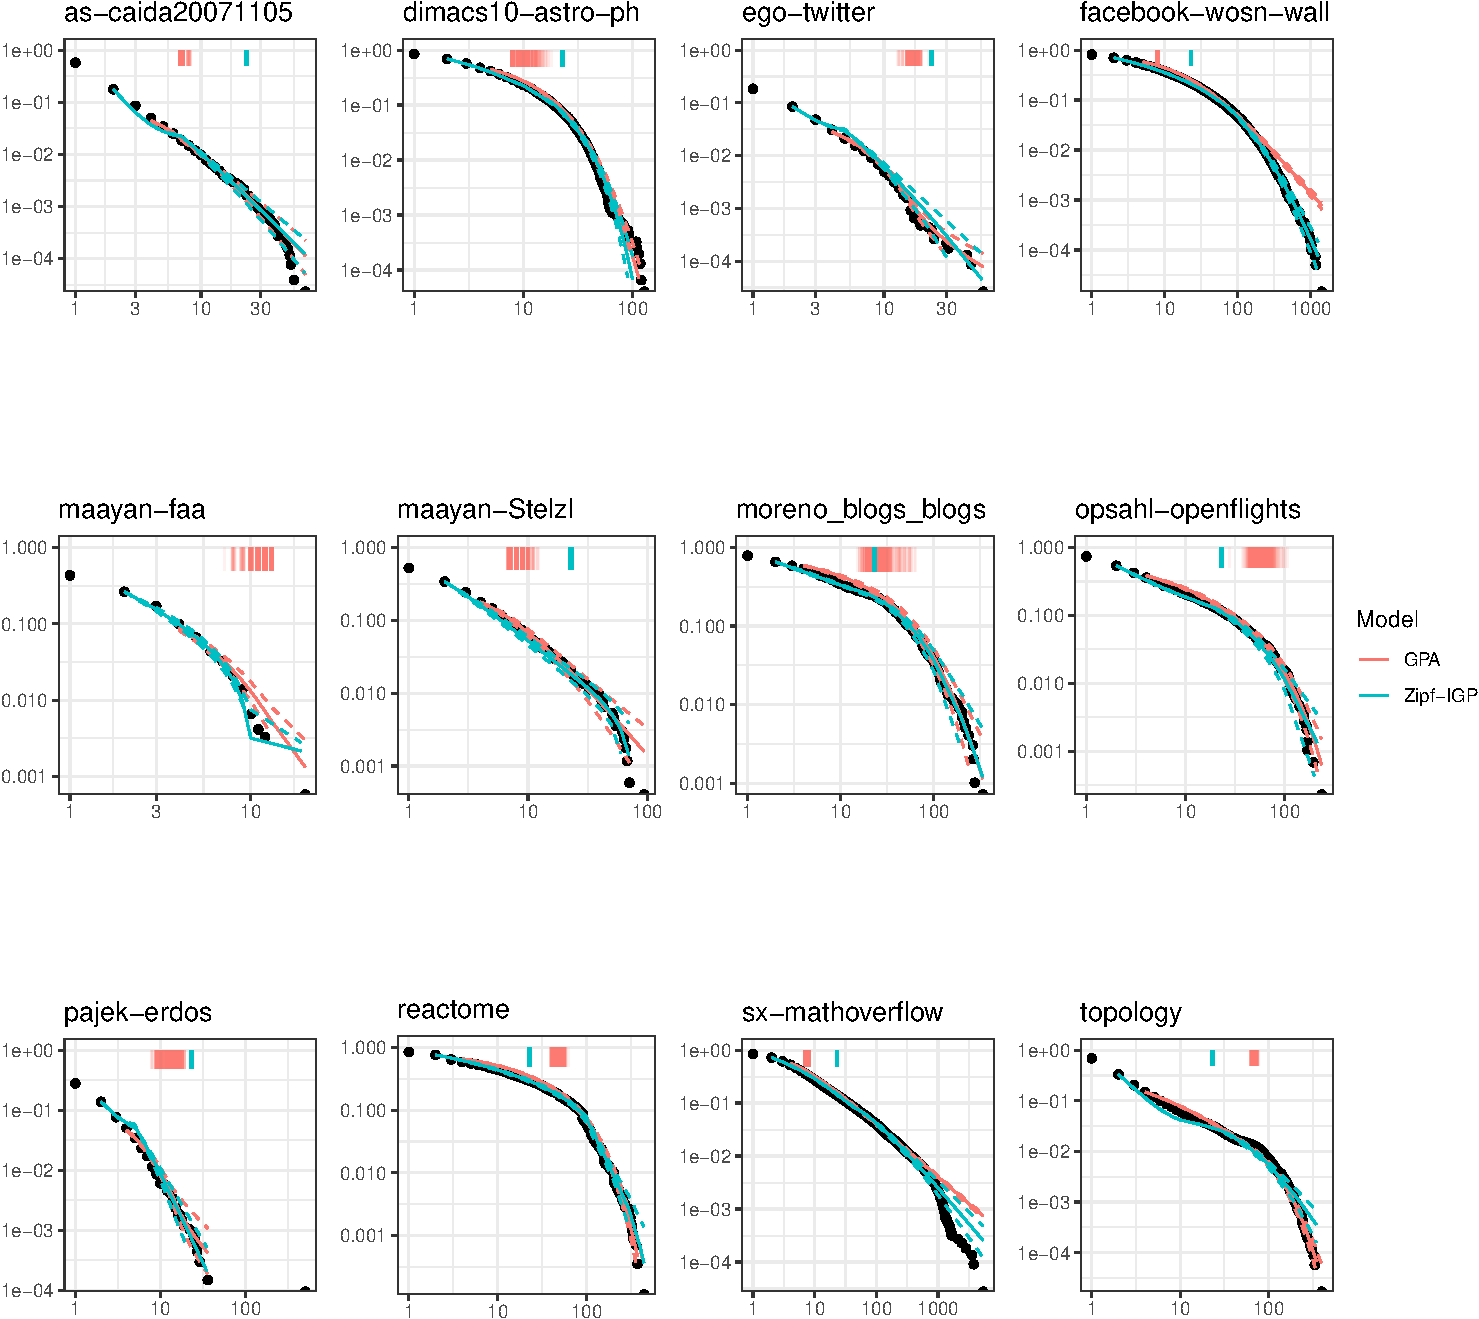
\includegraphics[width=0.8\linewidth,height=\textheight,keepaspectratio]{paper_files/figure-pdf/fig-real1-1.pdf}

}

\caption{\label{fig-real1}Posterior estimates (solid red) of survival
for several real data sets and their 95\% credible intervals (dotted
red)}

\end{figure}%

Figure~\ref{fig-real1} displays the posterior estimates of the survival
function for various data sets, obtained from fitting the GPA model and
the Zipf-IGP mixture model. In most cases, the GPA model does not
necessarily provide an improvement in fit when compared to the Zipf-IGP
model but where the GPA model fits well we gain additional information
about the preference function assuming that the network evolved
according the the GPA scheme. Figure~\ref{fig-shapes} shows the
posterior of the shape parameter \(\xi\) obtained from the Zipf-IGP
model alongside the posterior of the equivalent shape parameter
\(\beta/\lambda^*\) obtained from fitting the GPA model. Generally, the
GPA model performs similarly to the Zipf-IGP when estimating the tail
behaviour of the degree distribution and where it doesn't it appears to
either be because it is fitting better at the tail than the Zipf-IGP
model or because of the threshold being estimated as too low forcing
almost all of the data to be modelled by the linear part of the GPA.
This again shows the effects that small degrees have on this model,
which is somewhat expected as the theory used for this model is for
trees and none of these real networks (nor many real networks) are.

\begin{figure}[H]

\centering{

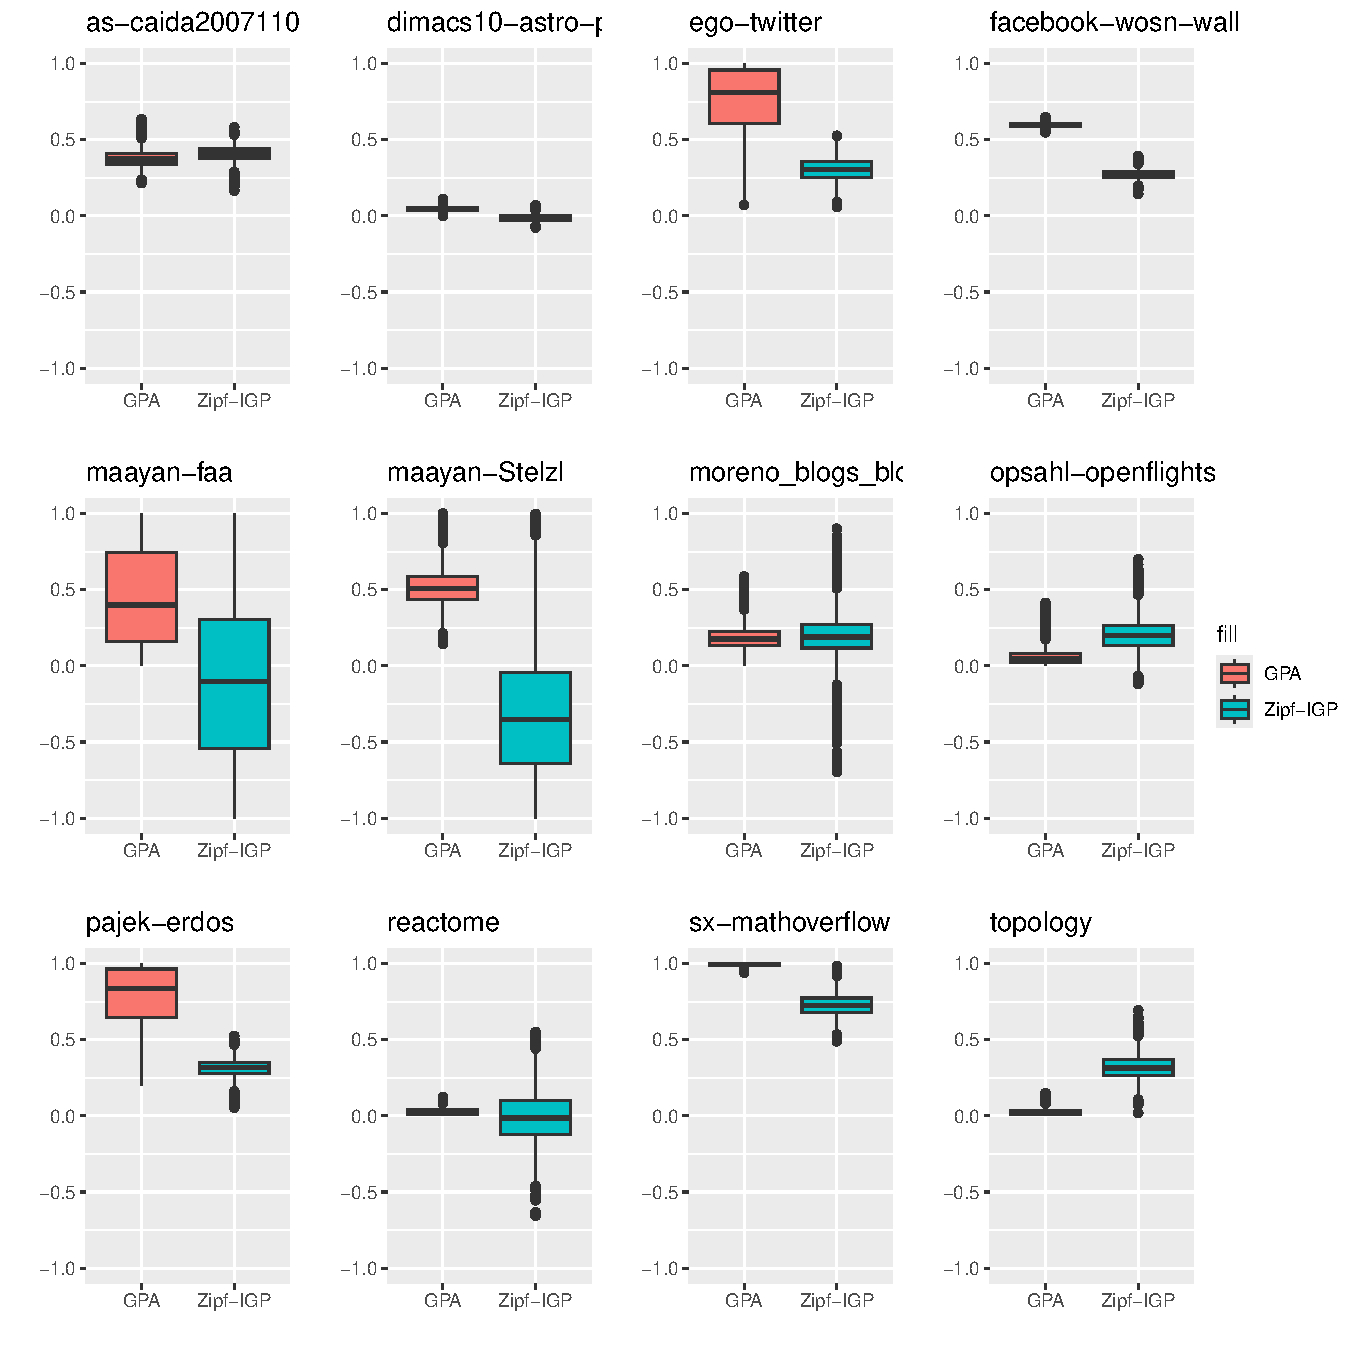
\includegraphics[width=0.8\linewidth,height=\textheight,keepaspectratio]{paper_files/figure-pdf/fig-shapes-1.pdf}

}

\caption{\label{fig-shapes}Posterior estimates (solid red) of survival
for several real data sets and their 95\% credible intervals (dotted
red)}

\end{figure}%

Figure~\ref{fig-pa} shows the estimated preference function \(b\)
alongside the 95\% credible interval on a log-log plot. Although the
credible interval becomes very large for the largest degrees, this is
expected as not all of these networks had data in that region, for those
that do the credible interval is much narrower as is the case for
\texttt{sx-mathoverflow}. The most insightful conclusion we can draw
from these plots come from the shape of the preference function. There
appears to be two distinct shapes of preference function. The first
appears mostly flat (similar to UA) for the smallest degrees and then
after a threshold PA kicks in, some with this shape are
\texttt{pajek-erdos} and \texttt{sx-mathoverflow}. The second distinct
shape appears provide some clear PA behaviour that then slows down after
a certain point, examples of this are seen in the two infrastructure
networks \texttt{opsahl-openflights} and \texttt{topology}.

\begin{figure}[H]

\centering{

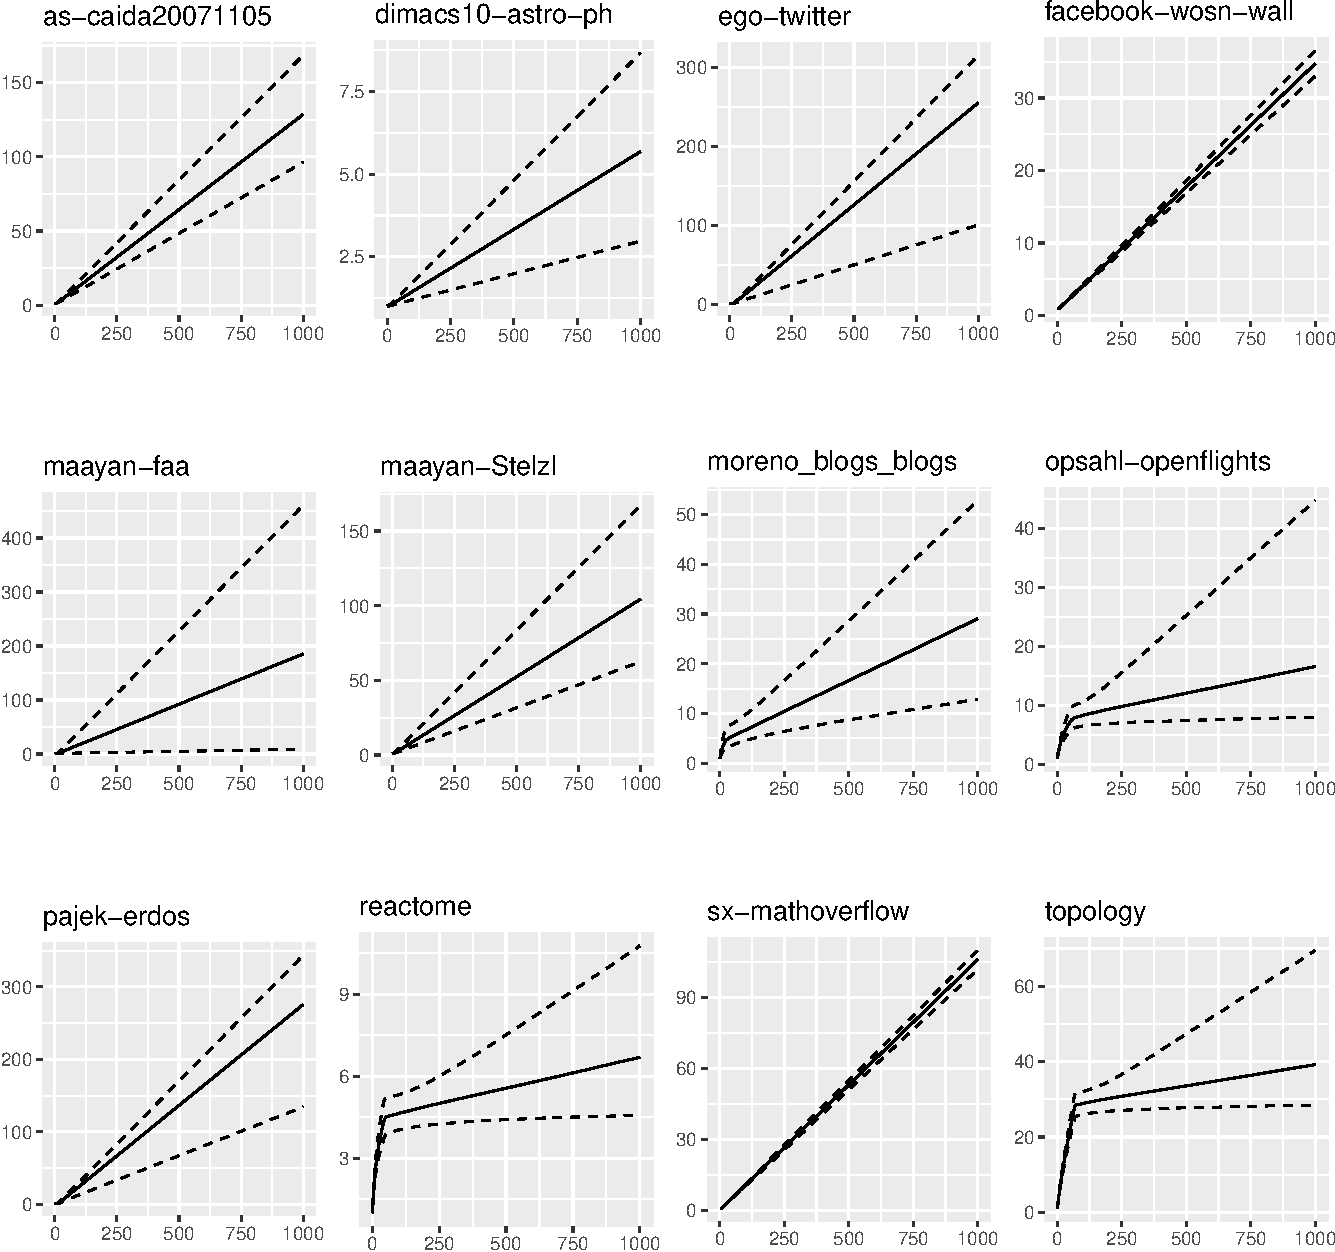
\includegraphics[width=0.8\linewidth,height=\textheight,keepaspectratio]{paper_files/figure-pdf/fig-pa-1.pdf}

}

\caption{\label{fig-pa}Posterior estimate for preference function
(solid) with 95\% credible interval (dashed) on log-log scale.}

\end{figure}%

\begin{figure}[H]

\centering{

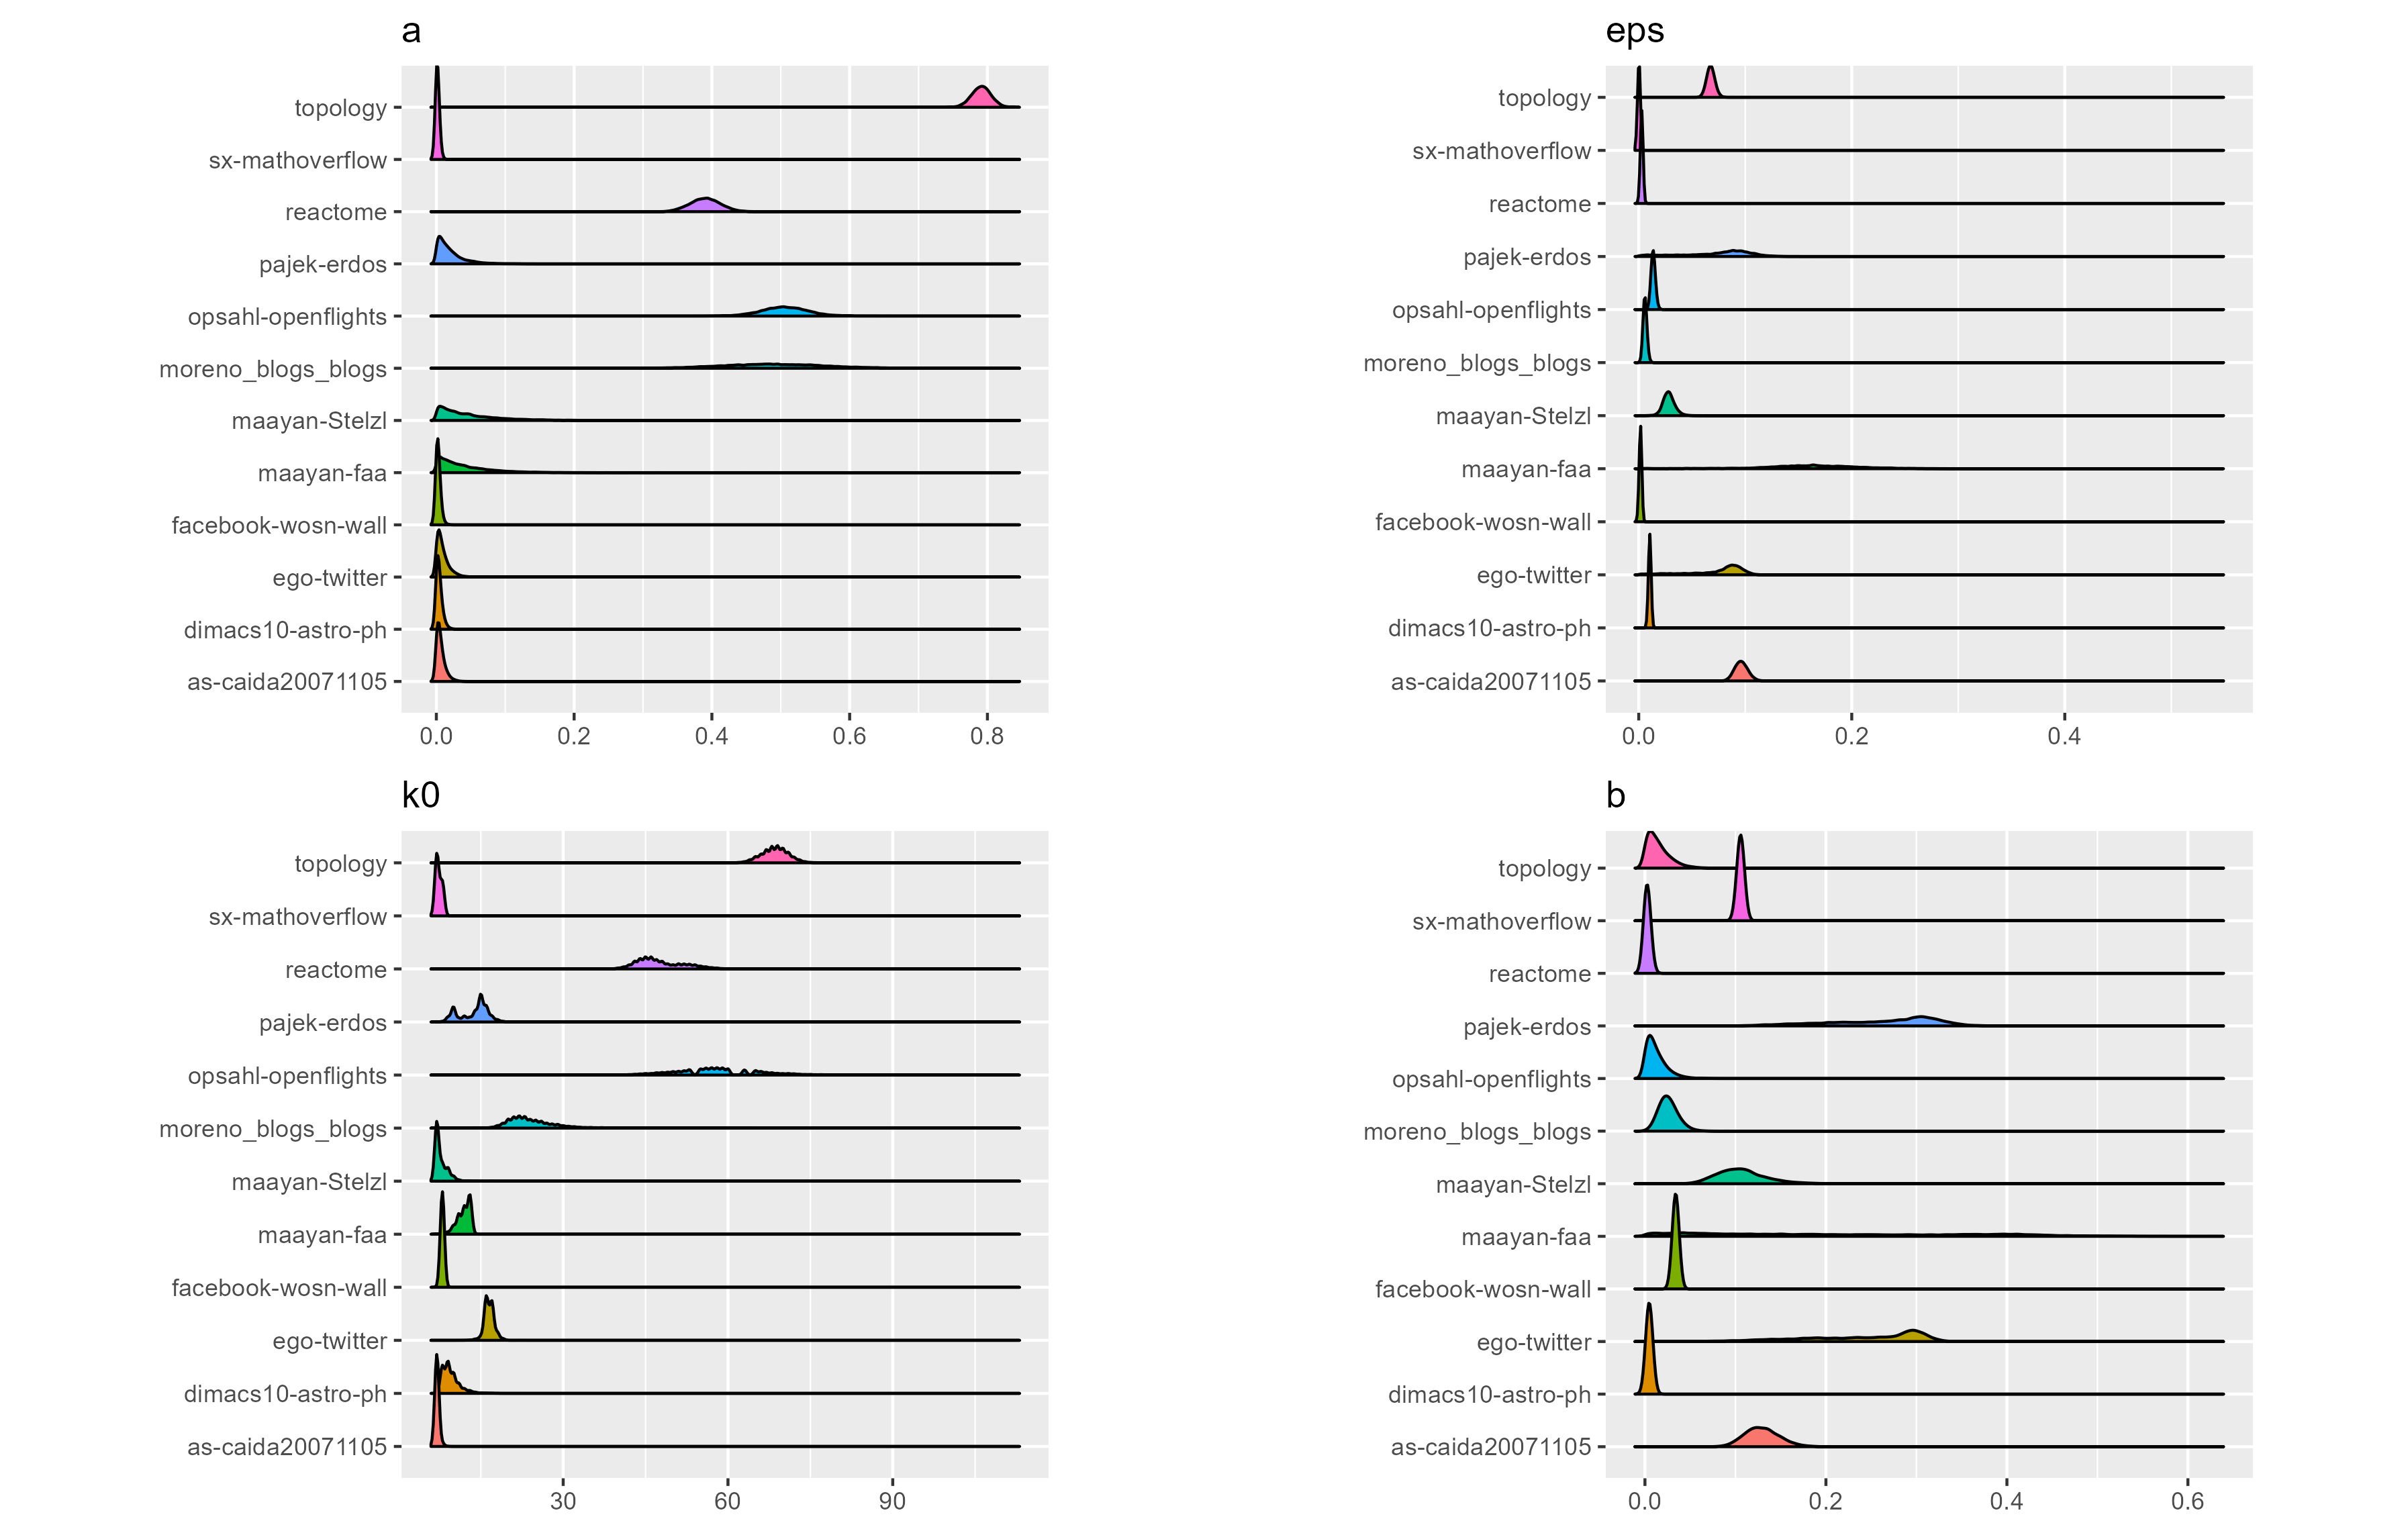
\includegraphics[width=0.8\linewidth,height=\textheight,keepaspectratio]{pars_plot.png}

}

\caption{\label{fig-rec3}Posterior estimates of parameters for real
data.}

\end{figure}%

\section{Conclusion and Discussion}\label{sec-conc}

In this paper we introduced a flexible class of preference function that
when used under the GPA scheme (in the tree setting) is guaranteed to
generate a network with a heavy tailed degree distribution whilst
remaining flexible in the body. Using simulations from networks using
this class of preference function we showed that the model parameters
are quite easily estimated from the degrees alone at a snapshot in time.
Seeing this we applied this method to the degree distributions of real
networks, estimating their model parameters assuming they evolved in the
same way. Not only did this yield fairly good fits for the degree
distribution, similar to that of the Zipf-IGP, it came with the added
benefit of giving a posterior estimate for a preference function.

Obviously this method had its flaws in that the lowest degrees needed to
be truncated as they had a very large effect on the fit of the model as
a result of using theory developed for trees and applying it to general
networks. Hopefully, as the field progresses we will be able to apply
theory developed for general networks using a similar method to this,
allowing us to compare the results here something that is more accurate.

GPA is also a fairly simplistic one on its own despite having large
flexibility in the preference function allowing for edges to only be
added at times when a new node is introduced into the network and not
allowing for anything like vertex/edge death, reciprocal edges and
rewiring steps. \citep{deijfen2015} introduces some theory for GPA with
vertex death based on the work by \citep{rudas07}, but is unable to come
to an expression for the degree distribution. However, adding something
like fitness scores into the GPA model seems fairly simple to do even
going so far as making each of the parameters used in the class of
functions here node-wise instead of universal. For example having the
preference weight for a vertex be given by
\(b(k_i, \underline{\gamma_i})\) where \(\underline{\gamma_i}\sim G\) is
the vertex's fitness and \(k_i\) is the vertex's degree, it is
reasonable to expect that the degree distribution for a model like this
to be given by:

\[
\bar F(k) = \mathbb E_G\left[\prod_{i=0}^k \frac{b(i, \gamma)}{\lambda^* + b(i,\gamma)}\right],\qquad \gamma\sim G,\, k=0,1,2,\ldots
\]

\section{Appendix}\label{appendix}

\subsection{Additional Results}\label{additional-results}

\subsubsection{Tail heaviness of general preferential attachment
model}\label{tail-heaviness-of-general-preferential-attachment-model}

Recall the limiting survival function:

\[
\bar F(k) = \prod_{i=0}^k \frac{b(i)}{\lambda^*+b(i)},
\]

The aim is to determine how this distribution behaves for different
choices of \(b\), specifically what maximum domain of attraction does
this distribution belong to and is it affected by the choice of
preference function \(b\). \citet{shimura12} introduces a quantity that
will help in determining what domain of attraction a discrete
distribution belongs to, that is:

For a distribution \(F\) with survival function \(\bar F\) and some
\(n\in\mathbb Z^+\) let:

\[
\Omega(F,n) = \left(\log\displaystyle\frac{\bar F (n+1)}{\bar F (n+2)}\right)^{-1} - \left(\log\displaystyle\frac{\bar F (n)}{\bar F (n+1)}\right)^{-1}
\]

\citep{shimura12} then states that if
\(\lim_{n\rightarrow\infty} \Omega(F,n) = 1/\alpha\) (\(\alpha>0\)),
then \(F\) is heavy tailed with \(\bar F(n) \sim n^{-\alpha}\).
Additionally, if \(\lim_{n\rightarrow\infty} \Omega(F,n) = 0\) then the
distribution is light tailed.

Consider a preference function \(b(\cdot)\) that fulfills:

\begin{equation}\phantomsection\label{eq-condb1}{
\lim_{n\rightarrow \infty} b(n) = \infty
}\end{equation}

Substituting in the form of \(\bar F(n)\) from \textbf{?@eq-surv} and
taking the limit, subject to Equation~\ref{eq-condb1}:

\begin{equation}\phantomsection\label{eq-omegares}{
\lim_{n\rightarrow\infty}\Omega(F,n) = \lim_{n\rightarrow\infty}\frac{b(n+2)-b(n+1)}{\lambda^*}.
}\end{equation} (see appendix for full proof).

Whilst there are many classes of functions that satisfy
Equation~\ref{eq-condb1} and Equation~\ref{eq-condb2}, the vast majority
of these result in \(\Omega(F,n) \rightarrow 0\), meaning that the
limiting degree distribution is light tailed. In fact, in order for the
limiting degree distribution to be heavy tailed, \(b\) must be
asymptotically linear (\(b(k)\sim k\)).

\subsection{Proofs}\label{proofs}

\subsubsection{Tail heaviness of GPA}\label{tail-heaviness-of-gpa}

Taking the form of the GPA degree survival: \[
\bar F(n) = \prod_{i=0}^n\frac{b(i)}{\lambda+b(i)}
\] and substituting into the formula for \(\Omega(F,n)\):

\begin{align*}
\Omega(F,n)&=\left(\log\frac{\prod_{i=0}^{n+1}\frac{b(i)}{\lambda+b(i)}}{\prod_{i=0}^{n+2}\frac{b(i)}{\lambda+b(i)}}\right)^{-1}-\left(\log\frac{\prod_{i=0}^{n}\frac{b(i)}{\lambda+b(i)}}{\prod_{i=0}^{n+1}\frac{b(i)}{\lambda+b(i)}}\right)^{-1}\\
&=\left(\log\frac{\lambda+b(n+2)}{b(n+2)}\right)^{-1}-\left(\log\frac{\lambda+b(n+1)}{b(n+1)}\right)^{-1}\\
&=\left(\log\left[1+\frac{\lambda}{b(n+2)}\right]\right)^{-1}-\left(\log\left[1+\frac{\lambda}{b(n+1)}\right]\right)^{-1}
\end{align*}

Clearly if \(b(n)=c\) or \(\lim_{n\rightarrow\infty}b(n)=c\) for some
\(c>0\) then \(\Omega(F,n)=0\). Now consider a non-constant \(b(n)\) and
re-write \(\Omega(F,n)\) as:

\begin{align*}
\Omega(F,n) &= \left(\log\left[1+\frac{\lambda}{b(n+2)}\right]\right)^{-1}-\frac{b(n+2)}{\lambda}+\frac{b(n+2)}{\lambda}-\left(\log\left[1+\frac{\lambda}{b(n+1)}\right]\right)^{-1}+\frac{b(n+1)}{\lambda}  -\frac{b(n+1)}{\lambda}\\
&=\left\{ \left(\log\left[1+\frac{\lambda}{b(n+2)}\right]\right)^{-1}-\frac{b(n+2)}{\lambda}\right\} - \left\{ \left(\log\left[1+\frac{\lambda}{b(n+1)}\right]\right)^{-1}-\frac{b(n+1)}{\lambda}\right\}+\frac{b(n+2)}{\lambda}-\frac{b(n+1)}{\lambda}
\end{align*}

Then if \(\lim_{n\rightarrow\infty}b(n)=\infty\) it follows that:

\begin{align*}
\lim_{n\rightarrow\infty}\Omega(F,n) &= \lim_{n\rightarrow\infty}\left\{ \left(\log\left[1+\frac{\lambda}{b(n+2)}\right]\right)^{-1}-\frac{b(n+2)}{\lambda}\right\} - \lim_{n\rightarrow\infty}\left\{ \left(\log\left[1+\frac{\lambda}{b(n+1)}\right]\right)^{-1}-\frac{b(n+1)}{\lambda}\right\}\\
&\qquad+\lim_{n\rightarrow\infty}\left(\frac{b(n+2)}{\lambda}-\frac{b(n+1)}{\lambda}\right)\\
&=\frac{1}{2}-\frac{1}{2} + \lim_{n\rightarrow\infty}\left(\frac{b(n+2)}{\lambda}-\frac{b(n+1)}{\lambda}\right)\\
&=\frac{1}{\lambda}\lim_{n\rightarrow\infty}\left[b(n+2)-b(n+1)\right]\qquad \square
\end{align*}

\subsubsection{Removing the infinite
sum}\label{removing-the-infinite-sum}

For a preference function of the form:

\[
b(k) = \begin{cases}
g(k),&k<k_0\\
g(k_0) + \beta(k-k_0), &k\ge k_0
\end{cases}
\] for \(\beta>0, k_0\in\mathbb N\) we have that

\begin{align*}
\hat\rho(\lambda) = \sum_{n=0}^\infty\prod_{i=0}^{n-1}\frac{b(i)}{\lambda+b(i)} &= \sum_{n=0}^{k_0}\prod_{i=0}^{n-1}\frac{g(i)}{\lambda+g(i)} + \sum_{n=k_0+1}^\infty\left(\prod_{i=0}^{k_0-1}\frac{g(i)}{\lambda+g(i)}\prod_{i=k_0}^{n-1}\frac{g(k_0) + \beta(i-k_0)}{\lambda +g(k_0) + \beta(i-k_0)}\right)\\
&=\sum_{n=0}^{k_0}\prod_{i=0}^{n-1}\frac{g(i)}{\lambda+g(i)} + \left(\prod_{i=0}^{k_0-1}\frac{g(i)}{\lambda+g(i)}\right)\sum_{n=k_0+1}^\infty\prod_{i=k_0}^{n-1}\frac{g(k_0) + \beta(i-k_0)}{\lambda +g(k_0) + \beta(i-k_0)}
\end{align*}

Now using the fact that:

\[
\prod_{i=0}^n(x+yi) = x^{n+1}\frac{\Gamma(\frac{x}{y}+n+1)}{\Gamma(\frac{x}{y})}
\] and reindexing the product in the second sum

\begin{align*}
\hat\rho(\lambda) &= \sum_{n=0}^{k_0}\prod_{i=0}^{n-1}\frac{g(i)}{\lambda+g(i)} + \left(\prod_{i=0}^{k_0-1}\frac{g(i)}{\lambda+g(i)}\right)\sum_{n=k_0+1}^\infty\frac{\Gamma\left(\frac{g(k_0)}{\beta}+n-k_0\right)\Gamma\left(\frac{\lambda+g(k_0)}{\beta}\right)}{\Gamma\left(\frac{\lambda+g(k_0)}{\beta}+n-k_0\right)\Gamma\left(\frac{g(k_0)}{\beta}\right)}\\
&= \sum_{n=0}^{k_0}\prod_{i=0}^{n-1}\frac{g(i)}{\lambda+g(i)} + \frac{\Gamma\left(\frac{\lambda+g(k_0)}{\beta}\right)}{\Gamma\left(\frac{g(k_0)}{\beta}\right)}\left(\prod_{i=0}^{k_0-1}\frac{g(i)}{\lambda+g(i)}\right)\sum_{n=k_0+1}^\infty\frac{\Gamma\left(\frac{g(k_0)}{\beta}+n-k_0\right)}{\Gamma\left(\frac{\lambda+g(k_0)}{\beta}+n-k_0\right)}\\
&=\sum_{n=0}^{k_0}\prod_{i=0}^{n-1}\frac{g(i)}{\lambda+g(i)} + \frac{\Gamma\left(\frac{\lambda+g(k_0)}{\beta}\right)}{\Gamma\left(\frac{g(k_0)}{\beta}\right)}\left(\prod_{i=0}^{k_0-1}\frac{g(i)}{\lambda+g(i)}\right)\sum_{n=1}^\infty\frac{\Gamma\left(\frac{g(k_0)}{\beta}+n\right)}{\Gamma\left(\frac{\lambda+g(k_0)}{\beta}+n\right)}
\end{align*}

In order to simplify the infinite sum, consider:

\begin{align*}
\sum_{n=0}^\infty\frac{\Gamma(n+x)}{\Gamma(n+x+y)} &=\frac{1}{\Gamma(y)}\sum_{n=0}^\infty \text{y}(n+x,y)\\
&=\frac{1}{\Gamma(y)}\sum_{n=0}^\infty\int_0^1t^{n+x-1}(1-t)^{y-1}at\\
&=\frac{1}{\Gamma(y)}\int_0^1 t^{x-1}(1-t)^{y-1}\sum_{n=0}^\infty t^n\,at\\
&=\frac{1}{\Gamma(y)}\int_0^1 t^{x-1}(1-t)^{y-1}\frac{1}{1-t}at\\
&=\frac{1}{\Gamma(y)}\int_0^1 t^{x-1}(1-t)^{y-2}at\\
&=\frac{1}{\Gamma(y)}\text{y}(x,y-1)\\
&= \frac{\Gamma(x)}{(y-1)\Gamma(x+y-1)}
\end{align*}

this infinite sum does not converge when \(x\le1\) as each term is
\(O(n^{-x})\). We can now use this in \(\hat\rho(\lambda)\):

\begin{align*}
\hat\rho(\lambda) &= \sum_{n=0}^{k_0}\prod_{i=0}^{n-1}\frac{g(i)}{\lambda+g(i)} + \frac{\Gamma\left(\frac{\lambda+g(k_0)}{\beta}\right)}{\Gamma\left(\frac{g(k_0)}{\beta}\right)}\left(\prod_{i=0}^{k_0-1}\frac{g(i)}{\lambda+g(i)}\right)\left(\frac{\Gamma\left(\frac{g(k_0)}{\beta}\right)}{\left(\frac{\lambda}{\beta}-1\right)\Gamma\left(\frac{g(k_0)+\lambda}{\beta}-1\right)}-\frac{\Gamma\left(\frac{g(k_0)}{\beta}\right)}{\Gamma\left(\frac{g(k_0)+\lambda}{\beta}\right)}\right)\\
&=\sum_{n=0}^{k_0}\prod_{i=0}^{n-1}\frac{g(i)}{\lambda+g(i)} + \left(\prod_{i=0}^{k_0-1}\frac{g(i)}{\lambda+g(i)}\right)\left(\frac{\Gamma\left(\frac{g(k_0)+\lambda}{\beta}\right)}{\left(\frac{\lambda}{\beta}-1\right)\Gamma\left(\frac{g(k_0)+\lambda}{\beta}-1\right)}-1\right)\\
&=\sum_{n=0}^{k_0}\prod_{i=0}^{n-1}\frac{g(i)}{\lambda+g(i)} + \left(\prod_{i=0}^{k_0-1}\frac{g(i)}{\lambda+g(i)}\right)\left(\frac{\frac{g(k_0)+\lambda}{\beta}-1}{\frac{\lambda}{\beta}-1}-1\right)\\
&=\sum_{n=0}^{k_0}\prod_{i=0}^{n-1}\frac{g(i)}{\lambda+g(i)} + \left(\prod_{i=0}^{k_0-1}\frac{g(i)}{\lambda+g(i)}\right)\left(\frac{g(k_0)+\lambda-\beta}{\lambda-\beta}-1\right)\\&=\sum_{n=0}^{k_0}\prod_{i=0}^{n-1}\frac{g(i)}{\lambda+g(i)} + \frac{g(k_0)}{\lambda-\beta}\prod_{i=0}^{k_0-1}\frac{g(i)}{\lambda+g(i)}\qquad \square
\end{align*}

\section{References}\label{references}

\renewcommand{\bibsection}{}
\bibliography{refs.bib}





\end{document}
